%^^^^^^^^^^^^^^^^^^^^^^^^^^^^^^^^^^^^^^^^^^^^^^^^^^^^^^^^^^^^^^^^^^^^^^^^^^^^^^^
% La rappresentazione 2D dello spazio delle configurazioni Cinematiche  a supporto compatto
% con aggiunta delle soluzioni della lagrangiana perturbata
%_______________________________________________________________________________

\documentclass{standalone}

%\usetikzlibrary{...}
\usepackage{tikz}
\usepackage{pgfplots}
\pgfplotsset{compat=newest}

%Common symbols
%Common math symbols
	%Number fields
		\newcommand{\Real}{\mathbb{R}}
		\newcommand{\Natural}{\mathbb{N}}
		\newcommand{\Relative}{\mathbb{Z}}
		\newcommand{\Rational}{\mathbb{Q}}
		\newcommand{\Complex}{\mathbb{C}}
	
%equality lingo
	%must be equal
		\newcommand{\mbeq}{\overset{!}{=}} 

% function
	%Domain
		\newcommand{\dom}{\mathrm{dom}}
	%Range
		\newcommand{\ran}{\mathrm{ran}}
	

% Set Theory
	% Power set (insieme delle parti
		\newcommand{\PowerSet}{\mathcal{P}}

%Differential Geometry
	% Atlas
		\newcommand{\Atlas}{\mathcal{A}}
	%support
		\newcommand{\supp}{\textrm{supp}}

	
	
%Category Theory
	%Mor set http://ncatlab.org/nlab/show/morphism
%		\newcommand{\hom}{\textrm{hom}}

%Geometric Lagrangian Mechanics
	% Kinematic Configurations
		\newcommand{\Conf}{\mathtt{C}}
	%Solutions Space
		\newcommand{\Sol}{\mathtt{Sol}}
	%Lagrangian class
		\newcommand{\Lag}{\mathsf{Lag}}
	%Lagrangiana
		\newcommand{\Lagrangian}{\mathcal{L}}
	%Data
		\newcommand{\Data}{\mathsf{Data}}
	%unique solution map
		\newcommand{\SolMap}{\mathbf{s}}
	%Classical Observables
		\newcommand{\Obs}{\mathcal{E}}	
	%Phase Space
		\newcommand{\Phase}{\mathcal{M}}	

		\
		
%Peierls (per non sbagliare più)
		\newcommand{\Pei}{Peierls}

\begin{document}
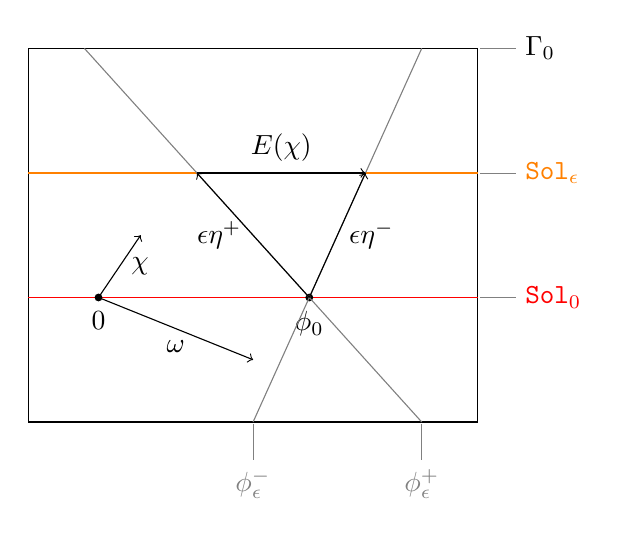
\begin{tikzpicture}
\begin{axis}[axis lines=none,clip=false]

	% Il riquadro di \Conf
	\addplot[color=black] coordinates {
		(8,6) (0,6) (0,0)(8,0)(8,6)
		}node [pos=1,pin={0:$\Gamma_0$},inner sep=0pt] {};

	% la retta di \Sol
	\addplot[color=red] coordinates {
		(0,2)
		(8,2)
	}node [pos=1,pin={0:$\Sol_0$},inner sep=0pt] {};
	
	% Zero section
	\node[label={270:{$0$}},circle,fill,inner sep=1pt] at (axis cs:1.25,2) {};
	% Fixed Solution
	\node[label={270:{$\phi_0$}},circle,fill,inner sep=1pt] at (axis cs:5,2) {};

	% La curva di \Sol_\epsilon
	\addplot[color=orange] coordinates {
	(0,4)(8,4)
	}node [pos=1,pin={0:$\Sol_\epsilon$},inner sep=0pt] {};

	%Variation
	\addplot[color=gray] coordinates {
		(1,6)
		(7,0)
	}node [pos=1,pin={270:$\phi_\epsilon^+$},inner sep=0pt] {};
	\addplot[color=gray] coordinates {
		(7,6)
		(4,0)
	}node [pos=1,pin={270:$\phi_\epsilon^-$},inner sep=0pt] {};
	
	%Perturbation
	\addplot[->] coordinates
           {(5,2) (3,4)}node [pos=0.5,label={180:$\epsilon \eta^+$},inner sep=0pt] {};
	\addplot[->] coordinates
           {(5,2) (6,4)}node [pos=0.5,label={0:$\epsilon \eta^-$},inner sep=0pt] {};

	%AdvancedMinusRetarded
	\addplot[->] coordinates
           {(3,4) (6,4)}node [pos=0.5,label={90:$E (\chi)$},inner sep=0pt] {};
           
	%LagrangianDensities
	\addplot[->] coordinates
           {(1.25,2) (4,1)}node [pos=0.5,label={270:$\omega$},inner sep=0pt] {};	
	\addplot[->] coordinates
           {(1.25,2) (2,3)}node [pos=0.5,label={0:$\chi$},inner sep=0pt] {};		
	
	

\end{axis}
\end{tikzpicture}
\end{document}